\documentclass[12pt]{article}
\usepackage[pdftex]{graphicx}

\oddsidemargin  -0.5 cm
\evensidemargin 0.0 cm
\textwidth      6.5in
\headheight     0.0in
\topmargin      -1 cm
\textheight=9.0in

\begin{document}

\section{Neutralinos to Two Leptons}

\begin{figure}[t]
  \begin{center}
    Electrons right-polarized 95\%, positrons unpolarized
    \begin{tabular}{p{0.49\linewidth} p{0.49\linewidth}}
      \begin{minipage}{\linewidth} 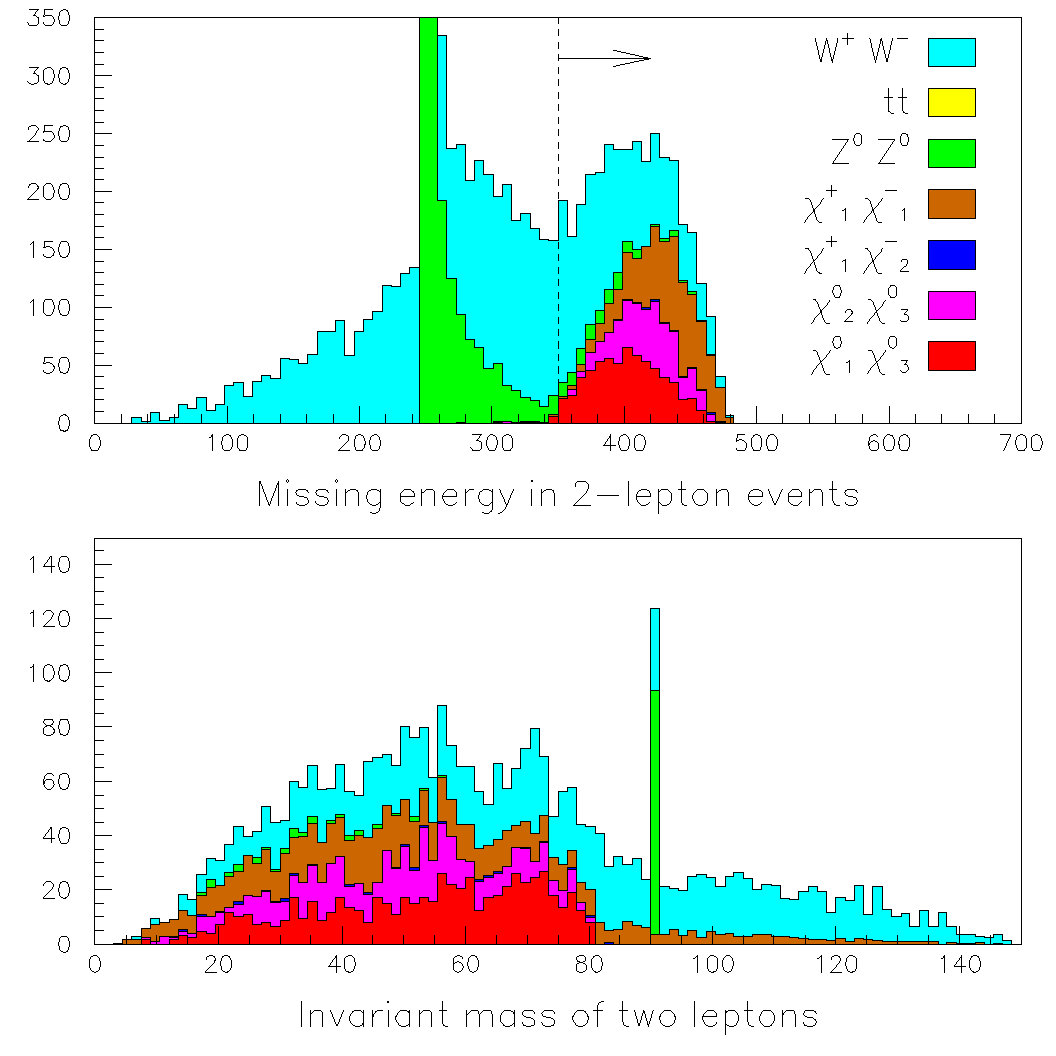
\includegraphics[width=\linewidth]{jimptwoleptons_a} \end{minipage} &
      \begin{minipage}{\linewidth} 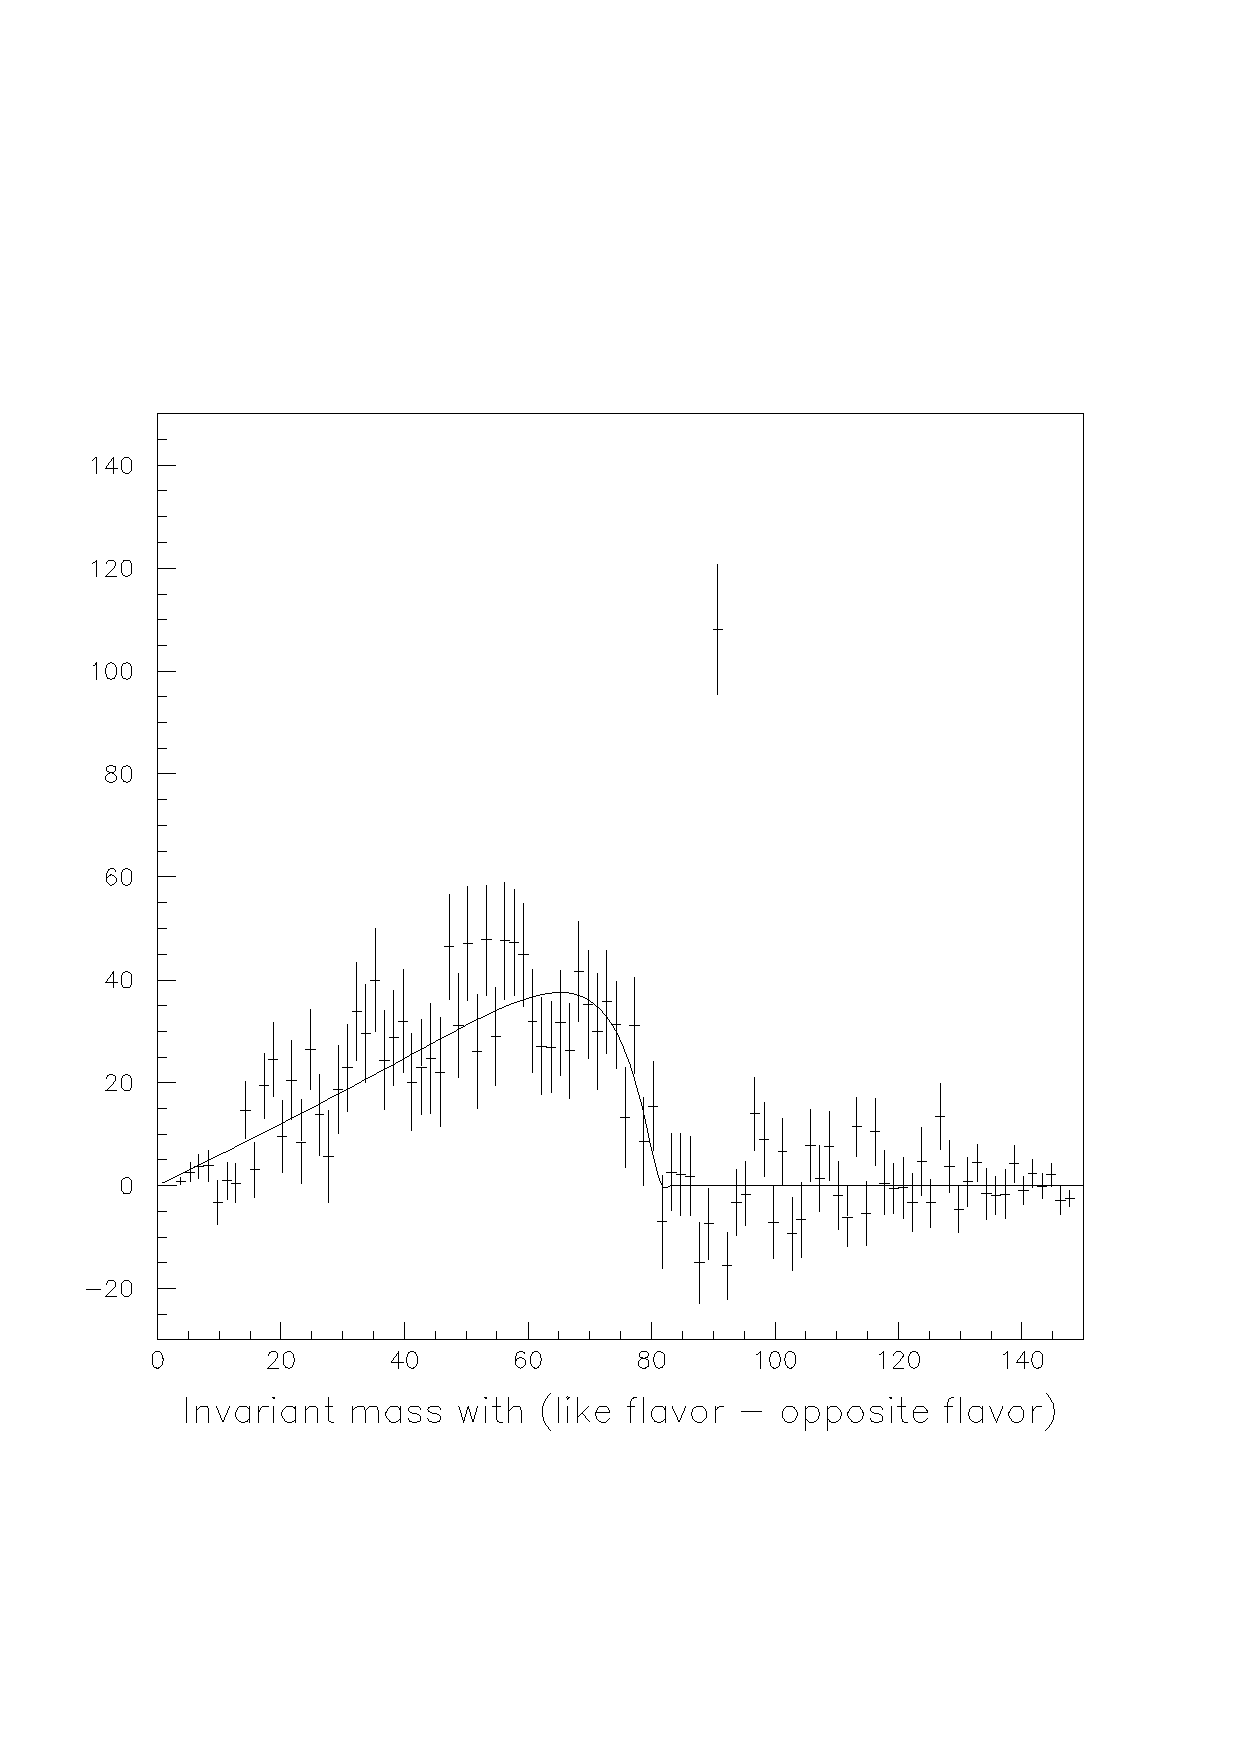
\includegraphics[width=\linewidth]{jimptwoleptons_b} \end{minipage}
    \end{tabular}

    \caption{Analysis of neutralinos from 250 fb$^{-1}$ of $e^+e^-$
    collisions: electrons 95\% right-polarized, positrons unpolarized.
    Left-top: Missing energy for events with zero jets and two tracks
    identified as leptons.  Left-bottom: Invariant mass of the two
    leptons with $>$ 350 GeV missing energy.  Right: Invariant mass
    with opposite-flavor leptons subtracted and fit to a threshold
    function.  (All Z-pair events are in the high bin at 91 GeV.)}

    \label{jimptwoleptons}
  \end{center}
\end{figure}

\begin{figure}[t]
  \begin{center}
    Electrons left-polarized 95\%, positrons unpolarized
    \begin{tabular}{p{0.49\linewidth} p{0.49\linewidth}}
      \begin{minipage}{\linewidth} 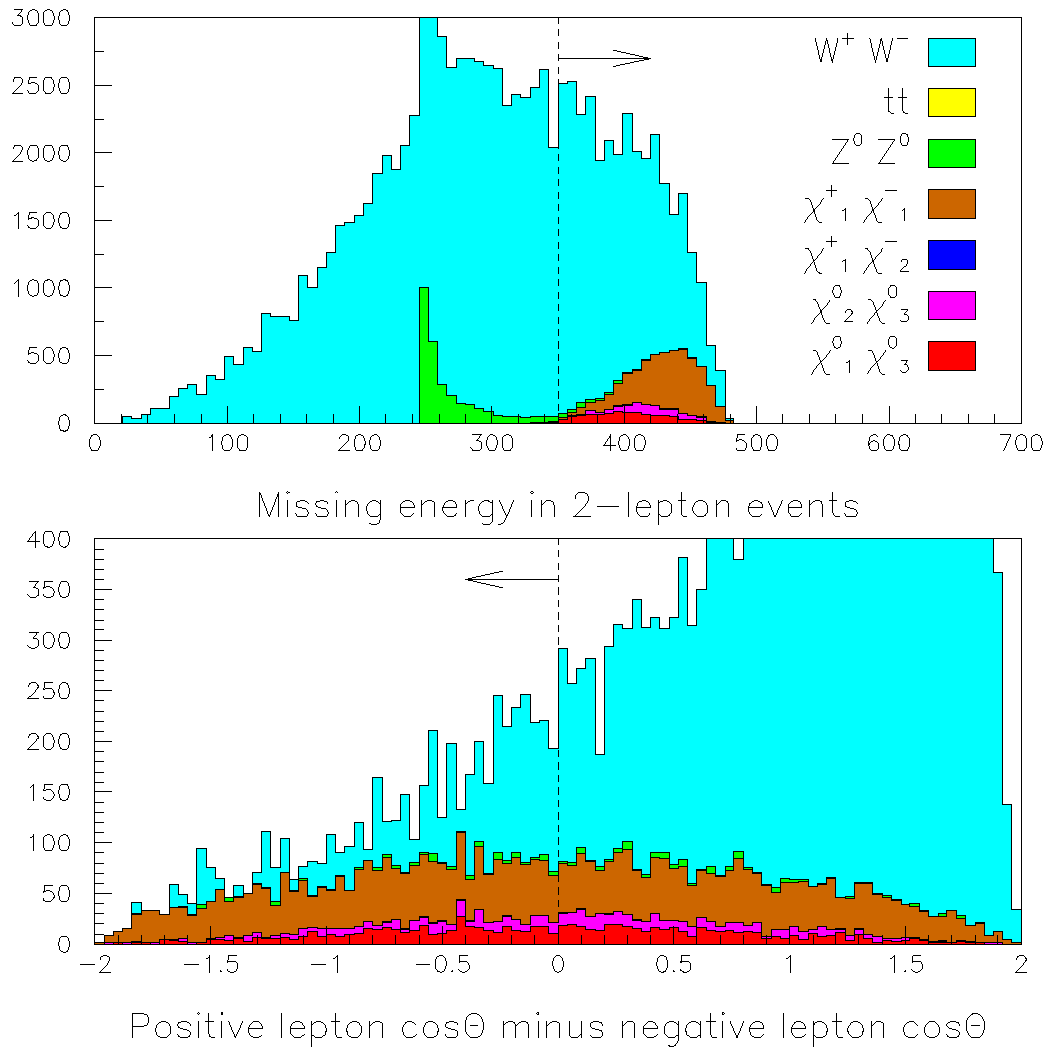
\includegraphics[width=\linewidth]{jimpleftleptons_a} \end{minipage} &
      \begin{minipage}{\linewidth} 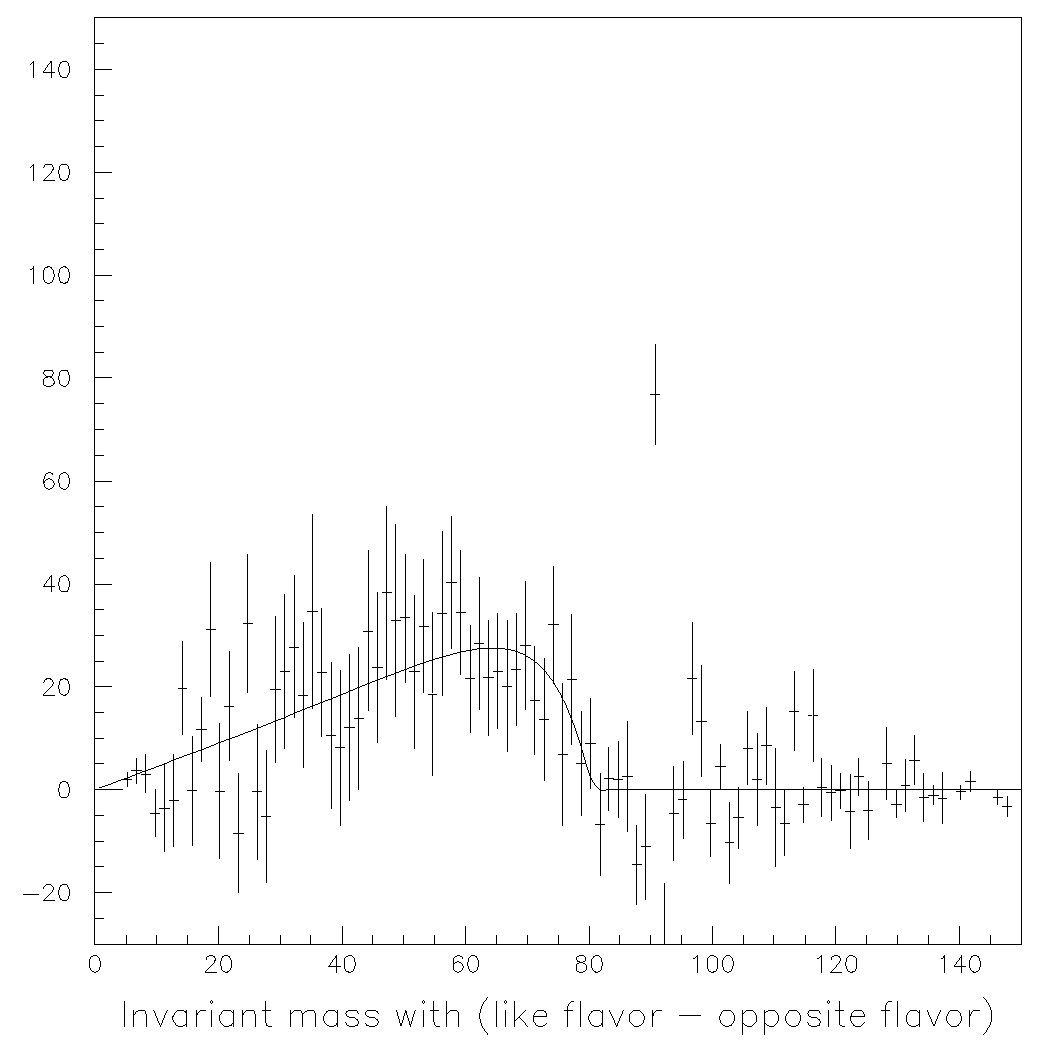
\includegraphics[width=\linewidth]{jimpleftleptons_b} \end{minipage}
    \end{tabular}

    \caption{Analysis of neutralinos from 250 fb$^{-1}$ of $e^+e^-$
    collisions: electrons 95\% left-polarized, positrons unpolarized.
    Left-top: Missing energy for events with zero jets and two tracks
    identified as leptons.  Left-bottom: Cosine of the polar angle of
    the positive track from the positron beam-line minus that of the
    negative track, with $>$ 350 GeV missing energy.  The cut at zero
    divides the signal symmetrically and avoids the region where
    $W^\pm$ is correlated in direction with the incident $e^\pm$.
    Right: Invariant mass with opposite-flavor leptons subtracted and
    fit to a threshold function, with missing energy and angle cuts
    applied.  (All Z-pair events are in the high bin at 91 GeV.)}

    \label{jimpleftleptons}
  \end{center}
\end{figure}

\begin{center}
  \begin{tabular}{l l l}
    $e^+e^- \to \tilde{\chi}^0_1$ & $\tilde{\chi}^0_3$ & \\
    & $\tilde{\chi}^0_3 \to \tilde{\chi}^0_1$ & $Z^*$ \\
    & & $Z^* \to \ell^+ \ell^-$
  \end{tabular}

\bigskip
and

\bigskip
  \begin{tabular}{l l l l l}
    $e^+e^- \to $ & $\tilde{\chi}^0_2$ & & $\tilde{\chi}^0_3$ & \\
    & $\tilde{\chi}^0_2 \to \tilde{\chi}^0_1$ & $Z^*$ & $\tilde{\chi}^0_3 \to \tilde{\chi}^0_1$ & $Z^*$ \\
    & & $Z^* \to \nu \bar{\nu}$ & & $Z^* \to \ell^+ \ell^-$
  \end{tabular}
\end{center}

\bigskip

Both neutralino modes, $\tilde{\chi}^0_1\tilde{\chi}^0_3$ and
$\tilde{\chi}^0_2\tilde{\chi}^0_3$, can be identified by selecting
events with two oppositely-charged tracks and missing energy.  This
lets the $\tilde{\chi}^0_3$ decay into a $Z^0 \to \ell^+\ell^-$ (two
electrons or muons) and $\tilde{\chi}^0_1$ (missing energy).  (The
prompt $\tilde{\chi}^0_1$ also contributes to missing energy.)  While
the neutralino signals can be cleanly distinguished from Standard
Model and chargino backgrounds, it is difficult to separate the two
signals from each other because $\tilde{\chi}^0_2$ can decay invisibly
into $\tilde{\chi}^0_1$ with a $Z^0 \to \nu \bar{\nu}$.  Consequently,
the two-lepton final state can only be used to measure a weighted sum
of the two modes, to be disambiguated later by the two jet, two lepton
measurement of $\tilde{\chi}^0_2\tilde{\chi}^0_3$ alone (see section
\ref{X}).  One measurement that is actually aided by the overlapping
modes is the mass difference between $\tilde{\chi}^0_3$ and
$\tilde{\chi}^0_1$; both neutralinos have an upper limit in invariant
mass at this mass difference.

The most effective means of background suppression comes from the
availability of polarized beams: if only the electron beam is 95\%
right-polarized, W-pair events in the signal region (missing energy)
are supressed by a factor of nine over unpolarized beams.  Although
the right-polarization will yield by far the most significant results,
we also consider the left-polarization, in which the W-pair background
is actually enhanced.

We select events with zero jets, two oppositely-charged tracks
identified as electrons or muons, and more than 350 GeV of missing
energy.  For a right-polarized beam, these are our only requirements
(Figure \ref{jimptwoleptons}).  For a left-polarized beam, swamped with
W-pair backgrounds, we also require that the polar angle of the
positive lepton with respect to the incident positron beam be less
than the polar angle of the negative lepton.  This avoids the region
in which the direction of the $W^\pm$ is correlated with the incident
$e^\pm$, reducing this background by more than a factor of ten.  The
neutralino signal, being forward-backward symmetric, is only reduced
by a factor of two (Figure \ref{jimpleftleptons}).

The primary backgrounds are W-pairs, Z-pairs, and light charginos.
W-pairs are either suppressed by right-polarization or the angular cut
described above, and Z-pairs have predictable missing energy outside
the regions of interest, leaving charginos as the only irreducible
background.  W-pairs and charginos can be subtracted without model
dependence by noting that signal neutralinos always decay to two
leptons of the same flavor, while W-pairs and charginos decay to two
uncorrelated lepton flavors.  (Each chargino decays to
$\tilde{\chi}^0_1$ with a $W^\pm$, which decays to a lepton and a
neutrino.)  If, therefore, we assume perfect flavor tagging and
subtract opposite-flavor events from the invariant mass plot, we
obtain a histogram with the two neutralino modes superimposed, W-pair
and chargino backgrounds only contributing to statistical error, and
all Z-pair events in one bin (91 GeV) above the maximum neutralino
invariant mass ($\sim$80 GeV).  These histograms are shown on the
rights of Figures \ref{jimptwoleptons} and \ref{jimpleftleptons}.

The combined cross-sections of $\tilde{\chi}^0_1\tilde{\chi}^0_3$ and
$\tilde{\chi}^0_2\tilde{\chi}^0_3$ can be determined by integrating
this histogram up to about 85 GeV (to exclude bias from the Z-pairs
and statistical error from the W-pair and chargino subtraction).  For
250 fb$^{-1}$, this yields 1093 $\pm$ 65 for a right-polarized beam
and 720 $\pm$ 91 for a left-polarized beam with the cuts described.
The coefficients for the weighted sum of cross-sections are derived
from branching fractions and efficiencies for each mode into the two
detected leptons with all applied cuts.  The branching fractions times
efficiencies are given in Table
\ref{jimpbetable}.

\begin{table}[!h]
  \begin{center}
    \renewcommand{\arraystretch}{1.5}
    \begin{tabular}{c c c}
      & electrons 95\% left-polarized & electrons 95\% right-polarized \\
      $\tilde{\chi}^0_1\tilde{\chi}^0_3$ & 0.0308 & 0.0584 \\
      $\tilde{\chi}^0_2\tilde{\chi}^0_3$ & 0.0123 & 0.0254
    \end{tabular}
    \renewcommand{\arraystretch}{1}
    \vspace{-0.5 cm}
  \end{center}

  \caption{Branching fractions times efficiencies for left- and
  right-polarized electron beams.  \label{jimpbetable}}

\end{table}

Dividing these by the number of events seen and multiplying by 250
fb$^{-1}$, we obtain the constraints on the left- and right-handed
cross-sections of $\tilde{\chi}^0_1\tilde{\chi}^0_3$ ($\sigma_{13}^L$
and $\sigma_{13}^R$) and $\tilde{\chi}^0_2\tilde{\chi}^0_3$
($\sigma_{23}^L$ and $\sigma_{23}^R$).
\begin{eqnarray}
  0.0107 \, \sigma_{13}^L + 0.00427 \, \sigma_{23}^L &=& 1 \pm 0.13 \, \sqrt{\frac{250 \mbox{ fb}^{-1}}{\mathcal{L}}} \\
  0.0133 \, \sigma_{13}^R + 0.00580 \, \sigma_{23}^R &=& 1 \pm 0.059 \, \sqrt{\frac{250 \mbox{ fb}^{-1}}{\mathcal{L}}}
\end{eqnarray}
where $\mathcal{L}$ is the total integrated luminosity.

Left- and right-polarized neutralino cross-sections are expected to
differ by about 30\%, but this difference will probably not be
observable.  Assuming a perfect $\sigma_{23}$ subtraction, the
difference between $\sigma_{13}^L$ (56.8 fb) and $\sigma_{13}^R$ (44.1
fb) can only be distinguished at the 3-$\sigma$ level with 900
fb$^{-1}$ of right-polarized collisions.

To measure the mass difference between $\tilde{\chi}^0_3$ and
$\tilde{\chi}^0_1$, we fit our lepton invariant mass spectrum to the
neutralino threshold function discussed in section \ref{Y}.  The
Z-pair bin contributes to the $\chi^2$ of the fit, but not any of its
derivatives near the minimum (since the fit function is exactly flat
at 91 GeV).  (It could just as easily be dropped from the fit.)  While
fits of this function to the histograms shown on the rights of Figures
\ref{jimptwoleptons} and \ref{jimpleftleptons} converged, they yielded
central values which depend linearly on the bin spacing for small
variations, even with five times as many bins!  For a different final
state (section \ref{Z}), this pathology is avoided by employing an
unbinned maximum likelihood fit, but such a technique would be hard to
implement without giving up the model-independent background
subtraction described above.  Since statistical errors should be
independent of the fitting technique, we report errors from our binned
$\chi^2$ minimization, which do not depend on bin spacing: $\pm$0.7
GeV from right-polarized electrons and $\pm$2 GeV from left-polarized
electrons.

\end{document}
